\documentclass[../EDF Master Thesis.tex]{subfiles}

\begin{document}
    Ein Teil der Aufgabenstellung beinhaltet das Erstellen von zwei Demo-Applikationen, welche die Funktion des \ac{edf}-Schedulers unter Beweis stellen.
    Die \ac{cpu}-Auslastung bezeichnet dabei, die theoretische Belegung der \ac{cpu}-Zeit von allen \ac{edf}-Tasks.

    \subsection{Blinky-Demo} \label{section:blinky_demo}
    Für eine optische Vorführung des \ac{edf}-Schedulers wurde eine 'Blinky-Demo' erstellt, welche drei \ac{edf}-Tasks beinhaltet.
    Jede der drei Tasks toggelt eine unterschiedliche \ac{led}, besitzt aber die gleichen \ac{edf} Parameter, welche in \autoref{table:blinky_demo_task_parameter} dargestellt sind.

    \begin{table}[ht!]
        \centering
        \begin{tabular}{l|c|c|c}
            Taskname & Periode & Deadline & \ac{wcet} \\
            \hline
            Task 1 & 50 & 100 & 100\\
            Task 2 & 50 & 100 & 100\\
            Task 3 & 50 & 100 & 100\\
        \end{tabular}
        \caption{Blinky-Demo Task Parameter}
        \label{table:blinky_demo_task_parameter}
    \end{table}

    Die drei Tasks wurden exakt so gewählt, dass sie die verschiedenen möglichen Status des \ac{edf}-Schedulers simulieren und optisch dargestellen werden.
    Der Benutzer kann mithilfe des integrierten Button auf dem STM32F769I-Disc0 Board die drei Tasks, wie in \autoref{fig:blinky_demo_ablaufdiagramm} zu sehen, erstellen und löschen.
    Eine \ac{cpu}-Auslastung über 100\% ist nicht möglich und führt somit zur Fehlerbehandlung aus \autoref{section:Fehlerbehandlung}.
    
    \begin{figure}[H]
        \centering
        \resizebox{0.61\textwidth}{!}{%
            \begin{tikzpicture}[node distance = 2cm, auto]
                % Place nodes
                \node [papProcess](pro1){Warten auf Benutzer};
                \node [papProcess, below = of pro1](pro2){Idle Task};
                \node [left = of pro2, xshift=-1cm](label21){Status 1};
                \node [right = of pro2, xshift=-1cm](label22){\small\parbox{4cm}{Button Counter: 1 \\\ac{cpu}-Auslastung: 0\%}};
                \node [papProcess, below = of pro2](pro3){Task 1 + Idle Task};
                \node [left = of pro3, xshift=-1cm](label31){Status 2};
                \node [right = of pro3, xshift=-1cm](label32){\small\parbox{4cm}{Button Counter: 2 \\\ac{cpu}-Auslastung: 50\%}};
                \node [papProcess, below = of pro3](pro4){Task 1 + Task 2};
                \node [left = of pro4, xshift=-1cm](label41){Status 3};
                \node [right = of pro4, xshift=-1cm](label42){\small\parbox{4cm}{Button Counter: 3 \\\ac{cpu}-Auslastung: 100\%}};
                \node [papProcess, below = of pro4](pro5){Task 1 + Task 2 + Task 3};
                \node [left = of pro5, xshift=-1cm](label51){Status 4};
                \node [right = of pro5, xshift=-1cm](label52){\small\parbox{4cm}{Button Counter: 4 \\\ac{cpu}-Auslastung: 150\%}};
                \node [papProcess, below = of pro5](pro6){Task 2 + Task 3};
                \node [left = of pro6, xshift=-1cm](label61){Status 5};
                \node [right = of pro6, xshift=-1cm](label62){\small\parbox{4cm}{Button Counter: 5 \\\ac{cpu}-Auslastung: 100\%}};
                \node [papProcess, below = of pro6](pro7){Task 3 + Idle Task};
                \node [left = of pro7, xshift=-1cm](label77){Status 6};
                \node [right = of pro7, xshift=-1cm](label72){\small\parbox{4cm}{Button Counter: 6 \\\ac{cpu}-Auslastung: 50\%}};
                % invisible node helpful later
                \node[left=1cm of pro6,scale=0.05](inv){};
            
                % Draw edges
                \path [line] (pro1) -- (pro2);
                \path [line] (pro2) -- (pro3);
                \path [line] (pro3) -- (pro4);
                \path [line] (pro4) -- (pro5);
                \path [line] (pro5) -- (pro6);
                \path [line] (pro6) -- (pro7);
                \path[-,draw] (pro7) -| node{} (inv.north);
                \path[line]{} (inv.north) |- node[above]{reset} (pro2);
            \end{tikzpicture}  
        }%
        \caption[Blinky-Demo Ablaufdiagramm]{Blinky-Demo Ablaufdiagramm (eigene Darstellung)}
        \label{fig:blinky_demo_ablaufdiagramm}
    \end{figure} 
    
    Die Eigenschaften der einzelnen Status aus \autoref{fig:blinky_demo_ablaufdiagramm} sind wie folgt:
    \begin{itemize}
        \item \textbf{Warten auf Benutzer}: Anfangs ist keine \ac{edf}-Task gestartet, die \ac{led}s leuchten dauerhaft und die Idle Task wird dauerhaft ausgeführt.
        \item \textbf{Status 1}: Sobald der Benutzer zum ersten Mal den Button drückt, wird 'Task 1' erstellt und ausgeführt.
            Nun blinkt die erste \ac{led} regelmäßig, die anderen beiden \ac{led}s leuchten weiterhin dauerhaft.
            Durch diese Konstellation teilen sich 'Task 1' und die Idle Task die \ac{cpu}-Zeit und es ergibt sich eine \ac{cpu}-Auslastung von 50\%.
        \item \textbf{Status 2}: Wird nun der Button ein zweites Mal gedrückt, wird 'Task 2' erstellt und es blinkt nun auch die zweite \ac{led} regelmäßig.
            Aufgrund der Taskparameter von 'Task 1' und 'Task 2' teilen sich die beiden Tasks nun die komplette \ac{cpu}-Zeit und lasten diese zu 100\% aus, dadurch wird die Idle Task nicht mehr ausgeführt.
        \item \textbf{Status 3}: Drückt der Benutzer nun ein drittes Mal den Button, wird 'Task 3' erstellt, die dritte \ac{led} fängt nun auch an zu blinken.
            Aufgrund der gewählten Taskparameter beträgt die \ac{cpu}-Auslastung nun 150\%, hier kann der \ac{edf}-Scheduler die einzelnen Deadlines nicht einhalten.
            Dies wird anhand der \ac{led}s sichtbar, da diese nun nur noch unregelmäßig blinken.
            Sofern der Debug Mode aktiviert ist, können die nicht eingehaltenen Deadlines der Tasks über die \ac{uart}-Schnittstelle sowie welche Task wie oft ihre Deadline verfehlt hat, ausgelesen werden.
        \item \textbf{Status 4}: Wird nun der Button ein weiteres Mal gedrückt, wird 'Task 1' gelöscht und die erste \ac{led} wird ausgeschaltet.
            Nun teilen sich 'Task 2' und 'Task 3' die \ac{cpu}-Zeit und die \ac{cpu}-Auslastung beträgt wieder 100\%, aus diesem Grund wird die Idle Task auch nicht aufgerufen.
        \item \textbf{Status 5}: Ein weiteres Drücken des Buttons löscht 'Task 2', nun teilen sich 'Task 3' und die Idle Task jeweils die hälfte der \ac{cpu}-Zeit.
        \item \textbf{Status 6}: Drückt der Benutzer nun ein weiteres Mal den Button wird 'Task 3' gelöscht und alle drei \ac{led}s leuchten dauerhaft.
            Die \ac{cpu}-Auslastung liegt nun bei 0\%, dadurch wird die Idle Task dauerhaft ausgeführt.
            Das System befindet sich nun wieder am Anfang der Ausführung und kann erneut die einzelnen Status ausführen.
    \end{itemize}

    \clearpage

    \subsection{\acf{fft}-Demo} \label{section:fft_demo}

        Die \ac{fft}-Demo erstellt und sendet mithilfe der erarbeiteten \ac{gui} auf dem Host-Computer alle 10ms ein Signal, bestehend aus einem oder mehreren Sinus- oder Kosinus-Signalen, an den Mikrocontroller über das \ac{udp}-Protokoll.
        Das Intervall von 10ms wurde so gewählt, dass eine ausreichend schnelle Aktualisierung und eine mittelmäßige Auslastung des Host-Computers gewährleistet ist.
        Dieses Intervall kann in der Konfiguration der \ac{fft}-Demo angepasst werden, jedoch sollte das Intervall nicht kleiner als 6ms gewählt werden, da die Summe der \ac{wcet} aller Tasks auf dem Mikrocontroller 6ms beträgt.
        Der Mikrocontroller führt, basierend auf dem empfangenen Signal, eine \ac{fft}-Berechnung aus und sendet die Ergebnisse an den Host-Computer zurück.
        Das Ablaufdiagramm mit allen Komponenten für die \ac{fft}-Demo ist in \autoref{fig:fft_demo_ablaufdiagramm} zu sehen.

        \begin{figure}[H]
            \centering
            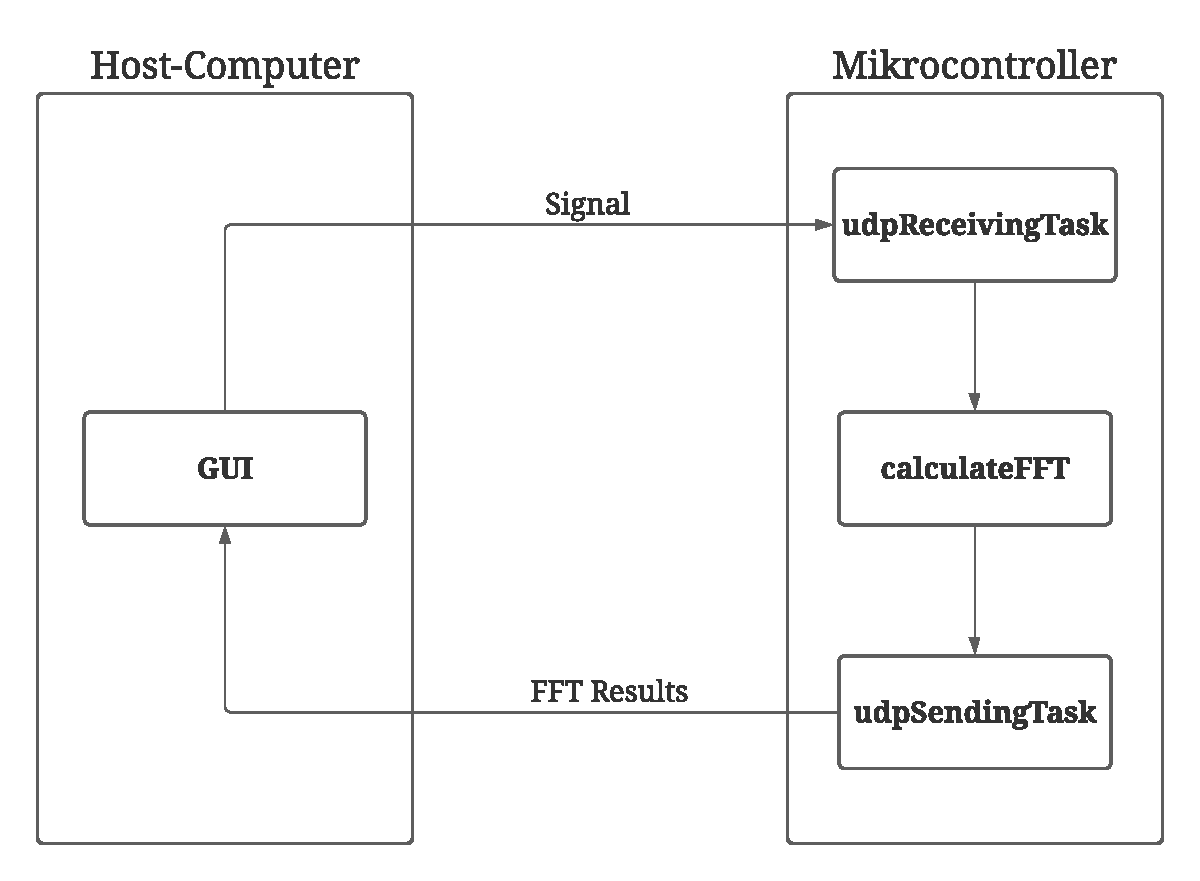
\includegraphics[height=10cm, width=14cm]{./attachments/FFT Ablauf.pdf}
            \caption[\ac{fft}-Demo Ablaufdiagramm]{\ac{fft}-Demo Ablaufdiagramm (eigene Darstellung)}
            \label{fig:fft_demo_ablaufdiagramm}
        \end{figure}

        Für das Erstellen und Senden eines Signals, des Empfangs der Ergebnisse und das Darstellen der Signale wurde eine \ac{gui}, basierend auf der Programmiersprache Python, erstellt.
        Des Weiteren wurden für die Kommunikation mit dem Host-Computer sowie die Berechnung der \ac{fft} drei \ac{edf}-Tasks erstellt.
        Das in dieser Arbeit generierte Signal wurde mit 2048 Abtastpunkten erzeugt und besitzt somit die gleiche Größe wie die verwendete \ac{fft}.
        Die Standard \ac{udp}-Paketgröße beträgt 1454 Bytes.
        Um 2048 Abtastpunkte von float-Werten (4 Byte) zu übermitteln, muss das Signal in mindestens 6 Pakete aufgeteilt werden.
        Jedoch besitzt das \ac{udp}-Protokoll keine Sortierfunktion, was bedeutet, falls ein Paket langsamer als das nächstfolgende Paket übertragen wird, würde dies zu einer Signalverfälschung führen.
        Aus diesem Grund wird bei jedem Paket auch die Paketnummer in einer Variable mit übertragen.
        Somit werden zur Übertragung von 2048 Abtastpunkten acht Pakte mit je 256 Samples übertragen.

        \clearpage

        \subsubsection{\acf{gui}}
            Die \ac{gui} wurde für eine einfache Bedienung sowie mit einer übersichtlichen Anzeige gestaltet und ist in \autoref{fig:grafische_benutzeroberflaeche} abgebildet.
            Dabei wurde auf eine einfache, flexible und übersichtliche Bedienung Rücksicht genommen.

            \begin{figure}[H]
                \centering
                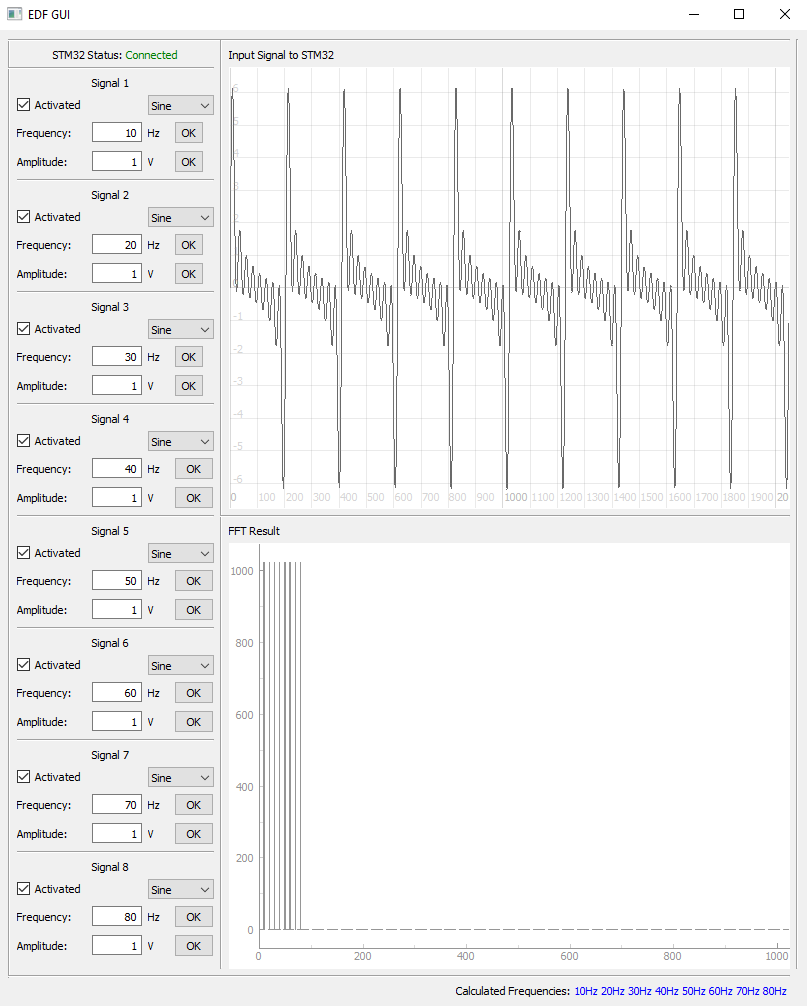
\includegraphics[width=0.92\textwidth]{./attachments/gui.png}
                \caption{Grafische Benutzeroberfläche der \ac{fft}-Demo}
                \label{fig:grafische_benutzeroberflaeche}
            \end{figure}

        In der linken oberen Ecke wird der Verbindungsstatus zum Mikrocontroller angezeigt, welcher mittels Pings von dem Host-Computer ermittelt wird.
        Unter dem Verbindungsstatus kann der Benutzer bis zu acht Signale aktiveren oder deaktivieren sowie auch deren Eigenschaften verändern.
        Das generierte Signal wird zentral in dem oberen Plotfenster dargestellt.
        Im unteren Plotfenster werden die Ergebnisse der \ac{fft}-Berechnung angezeigt, zusätzlich werden die erkannten Frequenzen in Textform unten eingeblendet.

        \subsubsection{Tasks des Mikrocontrollers}
            Die Perioden der drei \ac{edf}-Tasks, siehe \autoref{table:fft_demo_task_parameter}, wurden an das Intervall der \ac{gui} auf 10ms angepasst.
            Jede der drei Task hat einen \ac{wcet} von 2ms, welche mithilfe des Debugmodus ermittelt wurden, somit ergibt sich eine \ac{cpu}-Auslastung von 60\%, wie auch in \autoref{fig:fft_demo_task_scheduling} dargestellt.

            \begin{table}[ht!]
                \centering
                \begin{tabular}{l|c|c|c|l}
                    Taskname & Periode & Deadline & \ac{wcet} & Aufgabe \\
                    \hline
                    Task 1 & 10 & 10 & 2 & Empfangen des Signals über \ac{udp}\\
                    Task 2 & 10 & 10 & 2 & Berechnung der \ac{fft}\\
                    Task 3 & 10 & 10 & 2 & Senden der \ac{fft} Ergebnisse über \ac{udp}
                \end{tabular}
                \caption{\ac{fft}-Demo Task Parameter}
                \label{table:fft_demo_task_parameter}
            \end{table}

            Die \ac{wcet} ändern sich mit der Größe des empfangenen Signals und der Größe der \ac{fft}, jedoch wurden die Werte so gewählt, dass ein guter Kompromiss zwischen Arbeitsspeicherbelegung und Signalverarbeitung gewährleistet ist.
            Für die Implementierung der \ac{fft}-Demo ist es notwendig, dass die Tasks untereinander Daten austauschen können.
            Aus diesem Grund wurden \ac{freertos} Queues verwendet, damit die Tasks sich untereinander nicht blockieren können.

            \begin{figure}[H]
                \centering
                \sffamily
                \begin{tikzpicture}
                \begin{ganttchart}[%
                    hgrid,
                    inline, 
                    y unit title=1.1cm,
                    canvas/.style={draw=none},
                    title/.style={draw=none},
                    bar inline label anchor=west,
                    bar inline label node/.append style={anchor=west, text=white},
                    bar/.append style={fill=cyan!90!black}, 
                    bar height=1,
                    bar top shift = 0]{0}{19}
                \ganttbar[inline=false, bar/.append style={fill=blue!50}, bar label font=\color{blue!50}]{udpReceivingTask}{0}{1}
                \ganttbar[bar/.append style={fill=blue!50}]{}{10}{11}\\
                \ganttbar[inline=false, bar/.append style={fill=blue!70}, bar label font=\color{blue!70}]{calculateFFT}{2}{3}
                \ganttbar[bar/.append style={fill=blue!70}]{}{12}{13}\\
                \ganttbar[inline=false, bar/.append style={fill=blue!90}, bar label font=\color{blue!90}]{udpSendingTask}{4}{5}
                \ganttbar[bar/.append style={fill=blue!90}]{}{14}{15}\\
                \ganttbar[inline=false, bar label font=\color{cyan!90!black}]{Idle Task}{6}{9}
                \ganttbar[]{}{16}{19}\\
                \ganttvrule[vrule/.append style={red}]{Periode}{9}
                \ganttvrule[vrule/.append style={red}]{Periode}{19}
                \gantttitlelist[title label node/.append style={alias=n\x,opacity=0}]{0,...,19}{1}
                \end{ganttchart}
                \draw [-latex] (n0.north west) -- ([xshift=7pt]n19.north east) node[right] {$t$};
                \foreach \N in {0,...,19} {
                    \draw
                    let
                    \p1=(n0.center), \p2=(n1.center),\n1={(\x2-\x1)/2}
                    in
                    (n\N.north) +(-\n1,2pt) -- +(-\n1,-2pt) node[below,font=\small]{\N};
                }
                
                % draw tick for 19
                \draw
                    let
                    \p1=(n0.center), \p2=(n1.center),\n1={(\x2-\x1)/2}
                    in
                    (n19.north) +(\n1,2pt) -- +(\n1,-2pt) node[below,font=\small]{20};
                
                \end{tikzpicture}\\
                \caption[\ac{fft}-Demo Task Scheduling]{\ac{fft}-Demo Task Scheduling (eigene Darstellung)}
                \label{fig:fft_demo_task_scheduling}
            \end{figure}
\end{document}